\begin{figure}
\centering

\begin{tabular}{ l l l l l l } %    c}
	%                    label
	%  l            | l1   l2   l3   l4
	%  a   ---------+-------------------
	%  b   starting | a1 | a2 | a3 | a4
	%  e   strat    | b1 | b2 | b3 | b4
	%  l   ...
	& & \multicolumn{4}{c}{\textit{Strategy}} \\
	& 
		& %\parbox[c]{3cm}{
			\handmaxmin
			%} 
		& %\parbox[c]{3cm}{
			\handmaxavg
			%}
		& %\parbox[c]{3cm}{
			\handmaxposs
			%}
		& %\parbox[c]{3cm}{
			\handmaxmed
			%}
		\\
	%\cline{3-6}
	\multirow{7}{*}{
	\rotatebox{90}{
	\parbox[c]{6.5cm}{
		\textit{Starting Strategy}
	}
	}
	}
	%
	& \rotatebox[origin=c]{90}{\handmaxmin}
		&\parbox[c]{1em}{
\includegraphics[width=\stratgraphwidthmed]{images/findings/experiments/starting_points/matrix_handmaxmin_handmaxmin-7.png}}
		&\parbox[c]{1em}{
\includegraphics[width=\stratgraphwidthmed]{images/findings/experiments/starting_points/matrix_handmaxmin_handmaxavg-7.png}}
		&\parbox[c]{1em}{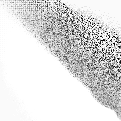
\includegraphics[width=\stratgraphwidthmed]{images/findings/experiments/starting_points/matrix_handmaxmin_handmaxposs-7.png}}
		&\parbox[c]{1em}{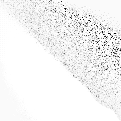
\includegraphics[width=\stratgraphwidthmed]{images/findings/experiments/starting_points/matrix_handmaxmin_handmaxmed-7.png}}
		%&
	\\ & & & & & \\
	%
	& \rotatebox[origin=c]{90}{\handmaxavg}
		&\parbox[c]{1em}{
\includegraphics[width=\stratgraphwidthmed]{images/findings/experiments/starting_points/matrix_handmaxavg_handmaxmin-7.png}}
		&\parbox[c]{1em}{
\includegraphics[width=\stratgraphwidthmed]{images/findings/experiments/starting_points/matrix_handmaxavg_handmaxavg-7.png}}
		&\parbox[c]{1em}{
\includegraphics[width=\stratgraphwidthmed]{images/findings/experiments/starting_points/matrix_handmaxavg_handmaxposs-7.png}}
		&\parbox[c]{1em}{
\includegraphics[width=\stratgraphwidthmed]{images/findings/experiments/starting_points/matrix_handmaxavg_handmaxmed-7.png}}
		%&\parbox[c]{1em}
	\\& & & & & \\
	%
	& \rotatebox[origin=c]{90}{\handmaxposs}
		&\parbox[c]{1em}{
\includegraphics[width=\stratgraphwidthmed]{images/findings/experiments/starting_points/matrix_handmaxposs_handmaxmin-7.png}}
		&\parbox[c]{1em}{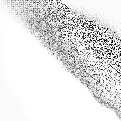
\includegraphics[width=\stratgraphwidthmed]{images/findings/experiments/starting_points/matrix_handmaxposs_handmaxavg-7.png}}
		&\parbox[c]{1em}{
\includegraphics[width=\stratgraphwidthmed]{images/findings/experiments/starting_points/matrix_handmaxposs_handmaxposs-7.png}}
		&\parbox[c]{1em}{
\includegraphics[width=\stratgraphwidthmed]{images/findings/experiments/starting_points/matrix_handmaxposs_handmaxmed-7.png}}
		%&\parbox[c]{1em}
	\\& & & & & \\
	%
	& \rotatebox[origin=c]{90}{\handmaxmed}
		&\parbox[c]{1em}{
\includegraphics[width=\stratgraphwidthmed]{images/findings/experiments/starting_points/matrix_handmaxmed_handmaxmin-7.png}}
		&\parbox[c]{1em}{
\includegraphics[width=\stratgraphwidthmed]{images/findings/experiments/starting_points/matrix_handmaxmed_handmaxavg-7.png}}
		&\parbox[c]{1em}{
\includegraphics[width=\stratgraphwidthmed]{images/findings/experiments/starting_points/matrix_handmaxmed_handmaxposs-7.png}}
		&\parbox[c]{1em}{
\includegraphics[width=\stratgraphwidthmed]{images/findings/experiments/starting_points/matrix_handmaxmed_handmaxmed-7.png}}
		%&\parbox[c]{1em}
	\\
\end{tabular}

\caption{
	Comparison of how different strategies develop with different
	starting points.
	The strategy along the \textit{Starting Strategy} axis is that strategy
	which started with 70\% weighting
	and the strategy along the \textit{Strategy} access is
	merely the strategy graph being presented.
	These strategy graphs are from an agent that has been trained for one
	million games
	against the same semi-pure strategy it started with,
	when playing as the dealer.
}
\label{fig:findings-expts-sanitycheck-matrix}
\end{figure}
